\chapter{Introduction}

\section{Motivation}
Wireless signal localization can be used in many areas, from surveillance to search and rescue \cite{wireless_loc}. In the past, these efforts have been focused largely on visual inspection. Increasingly, research has turned to using wireless signal localization to provide non line-of-sight solutions \cite{wireless_loc}. There are two major areas of research: the use of mass communication to inform people, and the use of new technologies to physically find people. This project focuses on the latter. There are new technologies emerging that are opening up new avenues for the location of people, namely low-cost, easy to use, highly maneuverable drones and cheap, powerful software defined radios (SDRs). \par
Drones and SDRs have very similar advantages in their respective industries: high flexibility and maneuverability at low costs. The motivation for this project is to integrate these technologies together to further enhance the state of the art in search, especially in areas with low visibility. Enabling a search of wireless signals opens the opportunity to locate sources otherwise impossible to locate. One such scenario would be a hiker lost in the Sierra Nevada forest with a cell phone, but no cell signal. Such a hiker would be nearly impossible to find visibly from a helicopter over the forest, but a drone with an SDR would be able to listen to beacons from their cell phone and calculate an approximation of their location as is depicted in Figure \ref{fig:sar_drone_forest}. \par
\begin{figure}[h!]
\centering
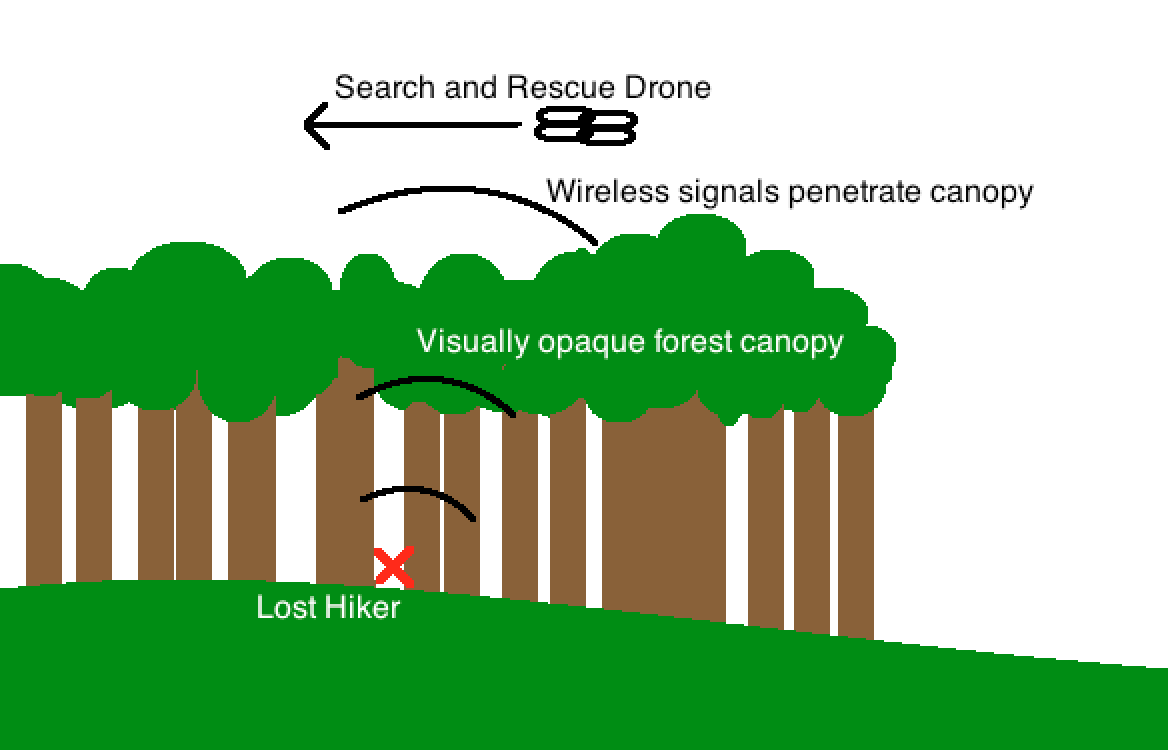
\includegraphics[width=0.70\textwidth]{img/sar_drone_forest}
\caption{Search and Rescue Drone flying above forest canopy to locate lost hiker via cell phone beacon signals. Wireless cell phone beacons penetrate the canopy while visual inspection is blocked.}
\label{fig:sar_drone_forest}
\end{figure}
Another example scenario is the issue of locating the controller of a non-cooperative drone. Visually, this would be very difficult, but being able to sense the controlling signal and locate the controller would be possible through the use of an SDR. A diagram of this scenario is included in Figure \ref{fig:locate_drone_crowd}. \par
\begin{figure}[h!]
\centering
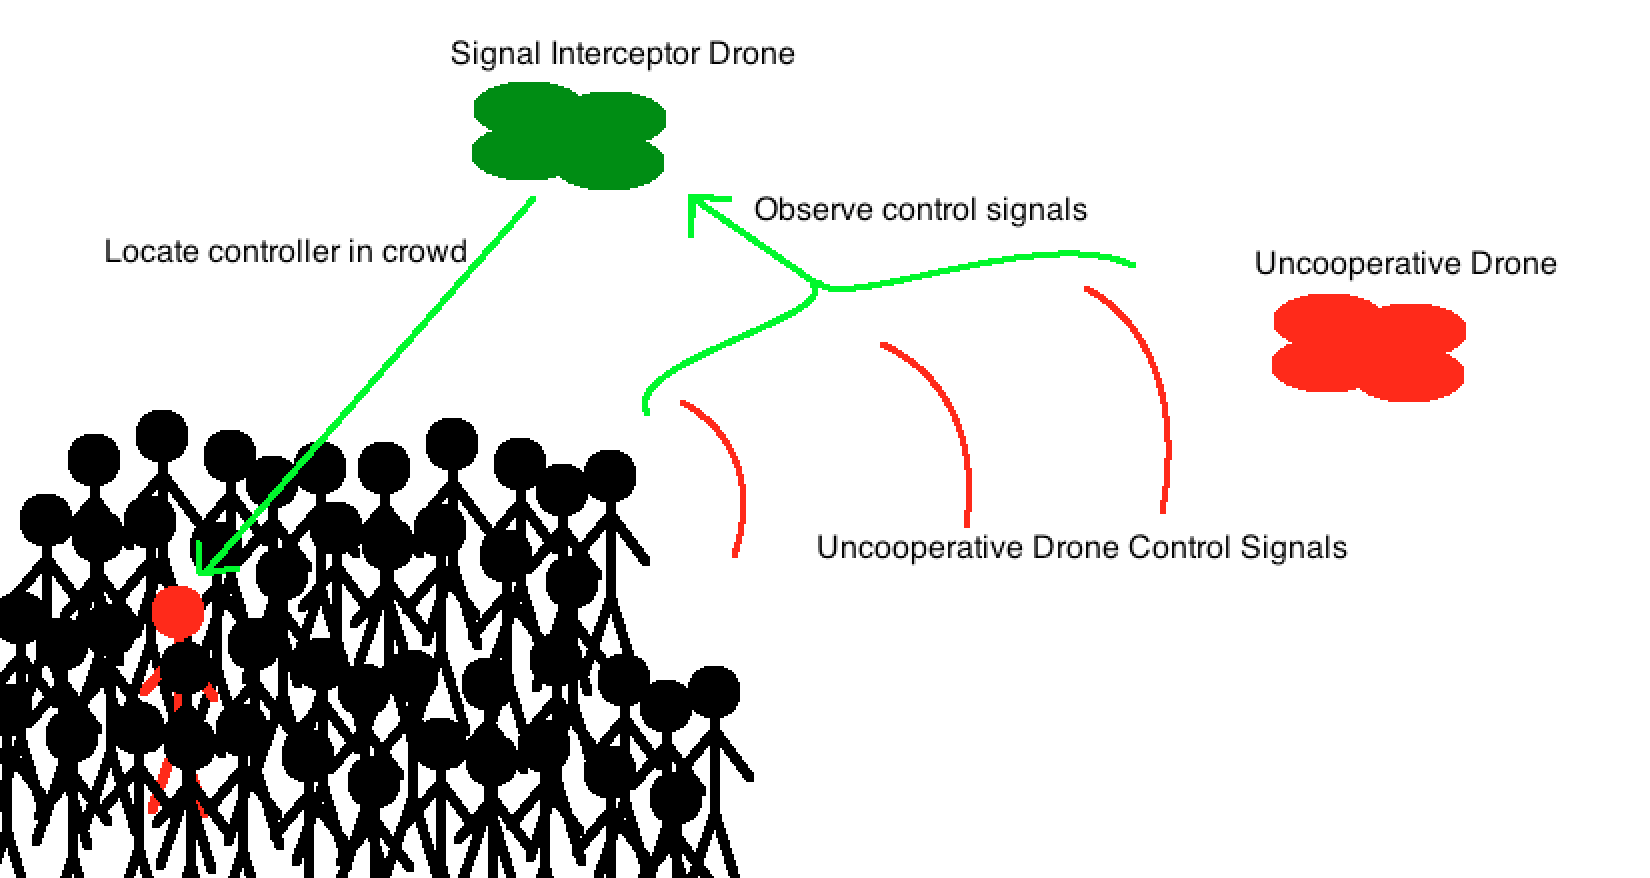
\includegraphics[width=0.70\textwidth]{img/locate_drone_controller}
\caption{Drone Controller Localization. Someone in a crowd is controlling an uncooperative drone that shouldn't be flying. The signal interceptor drone uses the control signals to locate where in the crowd the individual controlling the drone is.}
\label{fig:locate_drone_crowd}
\end{figure}

\section{Current State of the Art}
The advent of small, highly maneuverable drones has allowed the expansion of search capabilities to a finer scale with the use of mounted cameras. Low cost drones are also beginning to replace helicopters for traditional search and rescue missions \cite{drone_replacement}. The increased maneuverability and decreased cost is driving the movement toward drones.\par
Another quickly growing technology is the Software Defined Radio (SDR), which is easy to reconfigure \cite{int_radio}. This allows an SDR to receive and transmit a wide range of waveforms. Using SDRs, it’s possible to create an intelligent radio that can modify its own parameters to best match its environment \cite{int_radio}. SDRs have also been used in a passive listening configuration to create a radar receiver \cite{radar_conf}. The flexibility these radios provide over traditional hardware radios is perfect for any application that benefits from tuning to different frequencies, bandwidths, and modulation schemes.\par
Research in locating wireless emissions has produced some novel ideas using these new technologies. In a paper published in 2010, researchers note that more and more people have their cell phone on their person at all times. They investigate the detection of these phones by their wireless transmissions \cite{novel_localization}. In another research paper, the use of SDR hardware as a radar was investigated. Through the programmability of the SDR, the researcher was able to transmit and receive radar pulses with proper time and phase coherence, properties necessary to function as a radar receiver \cite{GNR_sdr}. There is no mention in the published literature, however, of combining SDR technology with drone technology.\par
\section{Proposed Design and Contributions}
The goal of this project is to assess and demonstrate the utility of an aerially maneuverable SDR by integrating a commercially available SDR with a low cost aerial drone. By taking advantage of a drone's maneuverability, a multitude of new sampling positions are reachable, resulting in higher accuracy for locating signal sources.\par

The design consists of a lightweight SDR connected to a directional multi-frequency antenna. The directionality of the antenna provides the opportunity for more accurate measurements: instead of simply measuring the signal strength at multiple points to triangulate, the platform is able to identify the strength and origin direction, reducing the number of points needed for the localization of a signal source, speeding up the process. Managing the SDR and sample processing is a single board computer (SBC), chosen for its balance between low weight, low power consumption, and ample processing power. In order to allow compatability with different drone platforms, the prototype will not explicitly communicate with its carrier drone, and will therefore include its own GPS receiver and other orientation sensors. This platform will henceforth be referred to as the Modular Aerial Software Defined Radio (MASDR) platform. This project adds to the state of the art by performing research into the combination of these two newly developed technologies. The findings from this project will provide new knowledge on the ability to localize wireless signals using an aerially mounted software defined radio. Creating this MASDR platform will open the door to many more discoveries and products through further more research and development. With more time to spend on software development, the MASDR platform would become much more capable in all aspects.\par
In addition to adding to the state of the art, this project seeks to develop a multipurpose platform which can be used for further research into the wireless spectrum from any location in the airspace. This could be used for channel modeling, heat mapping of wireless signals, and many more experiments into the behavior of various wireless signals in various environments.\par
\section{Report Organization}
This report is organized into seven chapters, the Introduction, Background, Proposed Approach, Methodology, Implementation, Results, and Conclusions. The Introduction presents the motivation for the project and the current state of the art to provide context for how this project relates to other prior and ongoing research. The Background chapter provides information on technologies and techniques used to make decisions and complete this project. In the Proposed Approach chapter, the report outlines the decision-making thought process for technical planning of the project. The Methodology chapter lays out the detailed plans of the project, its components, and the tests to verify functionality. The Methodology is followed by the Implementation chapter, which describes the implementation of the project in terms of hardware, software, and communications. In the Results chapter, the findings are presented organized by the test each finding came from. Finally, the Conclusions chapter summarizes the findings and provides recommendations for future work in the area.\par